\documentclass{standalone}
\usepackage{tikz}
\usepackage{ctex,siunitx}
\usepackage{tkz-euclide}
\usepackage{amsmath}
\usetikzlibrary{patterns, calc}
\usetikzlibrary {decorations.pathmorphing, decorations.pathreplacing, decorations.shapes,}
\begin{document}
\small
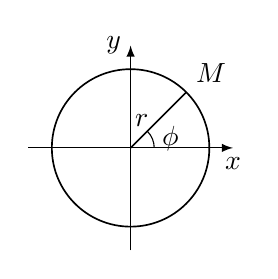
\begin{tikzpicture}[>=latex,scale=1.0]
  \tkzDefPoints{0/0/O}
  \draw[thin,->](-1.3,0)--(1.3,0)node[below]{$x$};
  \draw[thin,->](0,-1.3)--(0,1.3)node[left]{$y$};
  \draw[semithick](0,0)circle(1);
  \draw[semithick](0,0)--(45:1)node[midway,left]{$r$};
  \node at (45:1)[above right]{$M$};
  \draw[thin](0.3,0)arc(0:45:0.3)node[midway,right]{$\phi$};
\end{tikzpicture}
\end{document}